\section{Hint Generation}\label{section:hint-generation2}

Section~\ref{section:hint-generation1} introduced \tool's approach for providing easily accessible hints that facilitate the understanding of program errors and that can help to maintain students' motivation.

This section depicts how uncovered errors are logged, how hints are defined, and how matching hints are assigned to errors.

\subsection{Error Logging}

In order to allow teachers to tailor hints to the needs of their students, \tool logs program errors produced by learners. Whenever an error is raised during the execution of student-written code that is not covered by a hint yet, its error message is stored in the database.

Errors occurring during server-side code execution are immediately collected from the executing Docker container's standard error stream and are written to the database.

In contrast, errors raised during client-side execution must be collected in a different way. In order to intercept client-side errors, a handler for the \mintinline{js}{onerror}\foo{https://developer.mozilla.org/en-US/docs/Web/API/GlobalEventHandlers.onerror} \gls{dom} event is assigned to the pop-up window used for client-side rendering of submissions, for instance corresponding to student-written \gls{html} and other browser-renderable content. This handler serves as a global listener for any exception that is raised within the window. In this way, client-side errors can be intercepted, sent to the server, and stored in the database.

\subsection{Hint Definition}

Hints are defined by the teaching staff using \tool's administration back-end. Hints are matched to error messages using regular expressions since this allows ignoring minor textual differences resulting from context-specific information. While providing a regular expression, a hint's author can use subexpressions for matching concrete identifiers contained in an error message.

In Ruby, a \mintinline{rb}{NoMethodError}\foo{http://www.ruby-doc.org/core-2.1.5/NoMethodError.html} is raised whenever a method is called on a receiver that cannot handle it. This type of error is often caused by typing mistakes or falsely memorized method names.

\begin{listing}
\inputminted[frame=lines]{rb}{listings/hint-regular-expression.rb}
\vspace{-0.33cm}
\caption{Regular Expression for Matching \mintinline{rb}{NoMethodError} Instances}
\label{listing:hint-regular-expression}
\end{listing}

Listing~\ref{listing:hint-regular-expression} shows a regular expression to match \mintinline{rb}{NoMethodError} instances. It includes three subexpressions for matching the invoked method's name, the receiver's name, and the receiver's type.

\begin{listing}
\inputminted[frame=lines]{text}{listings/hint-message.txt}
\vspace{-0.33cm}
\caption{Hint Message for \mintinline{rb}{NoMethodError} Instances, Including Placeholders}
\label{listing:hint-message}
\end{listing}

Listing~\ref{listing:hint-message} displays a corresponding hint message, which contains three placeholders that match the regular expression's subexpressions. During hint generation, these placeholders are replaced by context-specific identifiers.

\subsection{Hint Matching}

\begin{figure}
\centering
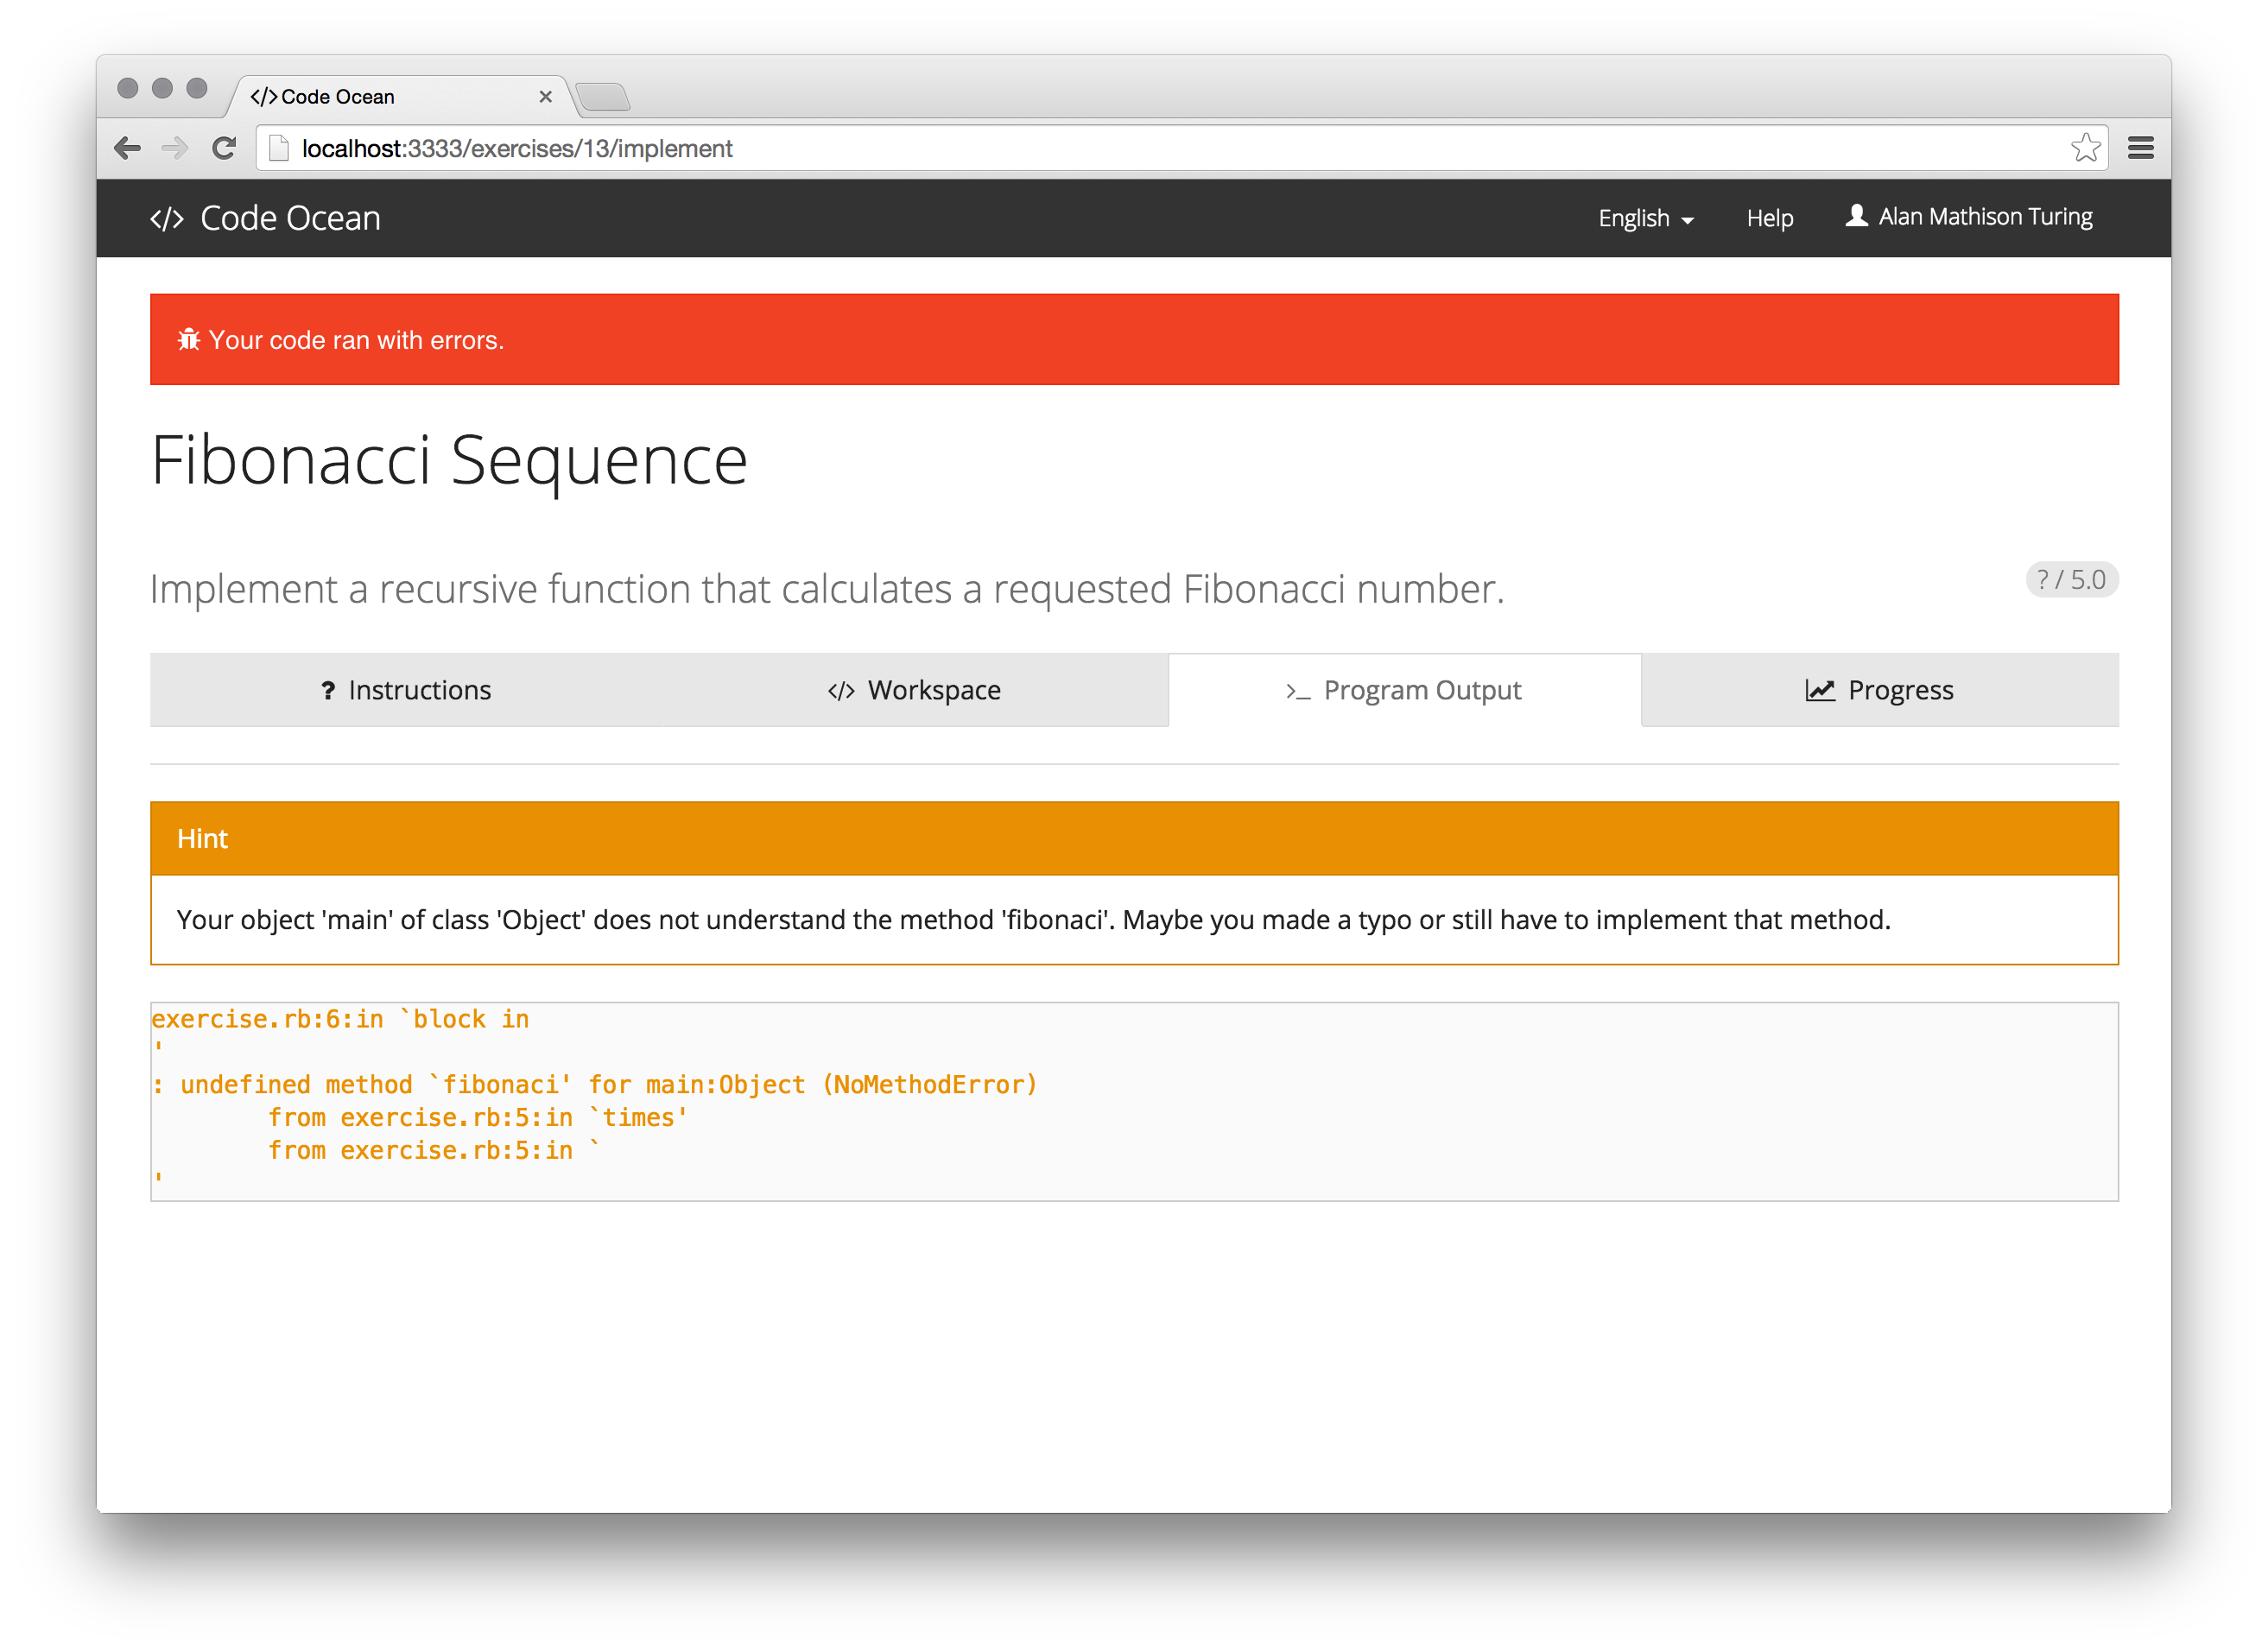
\includegraphics[width=\textwidth]{images/development-environment2.png}
\vspace{-1cm}
\caption{Development Environment: Hint Presentation}
\label{figure:development-environment2}
\end{figure}

Whenever an error occurs during the execution of student-written code, the error's message is matched against the regular expressions of all hints associated to the current execution environment. If a matching hint is found, its message is provided to the learner along with the original error message. Figure~\ref{figure:development-environment2} depicts how hints are presented to learners.

\begin{listing}
\inputminted[frame=lines]{text}{listings/hint-context-specific-message.txt}
\vspace{-0.33cm}
\caption{Concrete Hint Message for a Specific \mintinline{rb}{NoMethodError} Instance}
\label{listing:hint-context-specific-message}
\end{listing}

Provided that a hint's regular expression contains subexpressions, the hint's message is adapted to the actual context that the error occurred in by replacing placeholders with concrete identifiers extracted from the error message. Listing~\ref{listing:hint-context-specific-message} displays the hint message from Listing~\ref{listing:hint-message} after being adapted to an exemplary error context.

Maintaining original error messages and providing them along with hints enables learners to form a mental connection between errors and hints. Therefore, when confronted with an error of the same kind again, the learner might recall what she has learned.
